% Discussion (Josh). Moved from paper/vix_discussion.tex; headings demoted one level, preamble moved to main.tex.

\subsection{The VIX as the Market's ``Fear Gauge''}
\subsubsection{What the VIX measures}

The VIX is an index published by Cboe that measures the stock market's \emph{expected} volatility of the S\&P~500 over the next 30 calendar days. It is quoted in annualized percentage points. The VIX is \emph{forward-looking}: it is computed from the market prices of S\&P~500 index options, and is therefore a form of \emph{implied} volatility \cite{cboewp}. This is in contrast to historical (realized) volatility, which looks backward at past returns. 

Using the annualized convention, a VIX of $20$ corresponds to an expected one-standard-deviation move of the S\&P~500 over one month of about
\begin{equation}
  \frac{20\%}{\sqrt{12}} \approx 5.8\%.
\end{equation}

For a single option expiration with time to maturity $T$, Cboe calculates the annualized forward variance $\sigma^2$ as
\begin{equation}
  \sigma^2 = \frac{2}{T}\sum_i \frac{\Delta K_i}{K_i^2}\,e^{RT}\,Q(K_i)\;-\;\frac{1}{T}\left(\frac{F}{K_0}-1\right)^{2},
  \label{eq:vix-term}
\end{equation}
where:
\begin{itemize}
  \item $T$ is the time to expiration in calendar years, computed to the minute as $T = M / 525{,}600$, where $M$ is the number of minutes until settlement.
  \item $R$ is the risk-free interest rate to expiration (continuously compounded from Treasury yields).
  \item $F$ is the option-implied forward index level, derived from at-the-money put-call parity as $F = K^* + e^{RT}(C(K^*) - P(K^*))$, where $K^*$ is the strike minimizing $|C(K) - P(K)|$.
  \item $K_0$ is the strike price equal to or immediately below $F$.
  \item $K_i$ is the strike price of the $i$-th selected option. Out-of-the-money puts are used for $K_i < K_0$ and out-of-the-money calls for $K_i > K_0$.
  \item $Q(K_i)$ is the mid-quote price of the option at strike $K_i$. At $K_0$, both the call and put options are included, and $Q(K_0) = \frac{1}{2}\big(Q_{\text{put}}(K_0) + Q_{\text{call}}(K_0)\big)$.
  \item $\Delta K_i = \frac{1}{2}(K_{i+1} - K_{i-1})$ is the strike interval (with $\Delta K_1 = K_2 - K_1$ and $\Delta K_N = K_N - K_{N-1}$ at the truncation boundaries).
\end{itemize}

Because listed options rarely expire in exactly 30 days, Cboe selects two expirations bracketing 30 days (a near-term expiration $T_1$ and a next-term expiration $T_2$, with $23 < \text{days} < 37$) and computes $\sigma_1^2$ and $\sigma_2^2$ using~\eqref{eq:vix-term}. The 30-day spot VIX is then obtained via constant-maturity linear variance interpolation:
\begin{equation}
  \VIX = 100 \times \sqrt{ \left\{ T_1 \sigma_1^2 \left( \frac{N_{T_2} - N_{30}}{N_{T_2} - N_{T_1}} \right) + T_2 \sigma_2^2 \left( \frac{N_{30} - N_{T_1}}{N_{T_2} - N_{T_1}} \right) \right\} \frac{N_{365}}{N_{30}} },
  \label{eq:vix-interp}
\end{equation}
where $N_{T_1}$ and $N_{T_2}$ are the minutes to settlement for the two expirations, $N_{30} = 43{,}200$ minutes (30 days), and $N_{365} = 525{,}600$ minutes (365 days). The theoretical derivation of~\eqref{eq:vix-term} from variance-swap replication is presented in the pricing section of this report.


\subsubsection{Why it is called the fear gauge}

Investors who fear a market decline buy protection, typically out-of-the-money put options. Higher demand raises option prices and thus implied volatility. Equity returns and the VIX are strongly negatively correlated: the VIX tends to rise sharply when the S\&P~500 falls, and to drift lower in calm, rising markets. This asymmetry explains why VIX products are attractive as portfolio hedges.

Typical levels are roughly 10--15 in calm markets, a long-run average near 19--20, and readings well above 40 in crises such as late 2008 and March 2020 \cite{whaley}.

\begin{figure}[H]
  \centering
  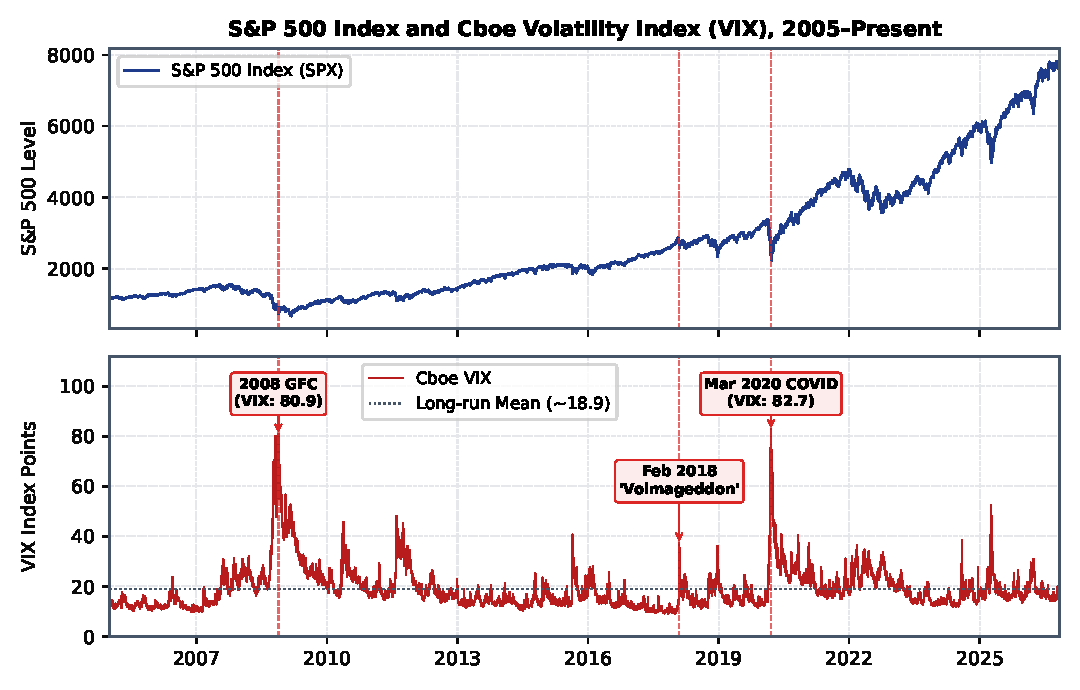
\includegraphics[width=0.9\linewidth]{figures/vix_vs_spx.pdf}
  \caption{S\&P~500 (top) and VIX (bottom), daily closes, January 2005 -- November 2026. Dotted lines mark 20 November 2008, 5 February 2018, and 16 March 2020; the dashed line is the average VIX over the period. Data: Yahoo Finance (\texttt{\textasciicircum GSPC}, \texttt{\textasciicircum VIX}).}
  \label{fig:vix-spx}
\end{figure}

\subsection{Trading Volatility Directly}
\subsubsection{Why volatility is hard to trade}

The VIX is a calculation, not a tradable asset: it cannot be bought, stored or delivered. Before volatility derivatives existed, investors could gain exposure to volatility only indirectly, for instance through delta-hedged option positions, which require continual rebalancing and carry other risks. Listed volatility products give a \emph{direct} and cheap way to take a view on volatility itself.

\subsubsection{The VIX product family}

Cboe introduced the VIX in 1993, adopted the current option-based methodology in 2003, launched VIX futures in 2004 and VIX options in 2006 \cite{cboewp}. Exchange-traded products linked to VIX futures followed from 2009 onward \cite{vxx}. Table~\ref{tab:products} summarizes the main instruments.

\begin{table}[H]
\centering
\small
\begin{tabular}{@{}p{3.4cm}p{3.6cm}p{3.6cm}p{4.2cm}@{}}
\toprule
\textbf{Product} & \textbf{Type} & \textbf{Underlying} & \textbf{Typical use}\\
\midrule
VIX Futures (\texttt{VX}) & Exchange-traded futures & Spot VIX at settlement & Portfolio hedging, directional speculation\\
\addlinespace
VIX Options & European cash-settled options & Spot VIX at settlement & Tail-risk hedging, asymmetric volatility bets\\
\addlinespace
Long VIX ETPs (\texttt{VXX}) & Exchange-traded note / fund & Rolling short-term VIX futures & Tactical short-term crash protection\\
\addlinespace
Inverse VIX ETPs (\texttt{SVXY}, \texttt{XIV}) & Inverse ETN / ETF & Rolling short VIX futures (daily reset) & Harvesting volatility risk premium\\
\addlinespace
Leveraged VIX ETPs (\texttt{UVXY}) & Leveraged ETN / ETF & Rolling leveraged VIX futures (daily reset) & Magnified short-term volatility exposure\\
\bottomrule
\end{tabular}
\caption{Overview of VIX-linked products.}
\label{tab:products}
\end{table}

\subsubsection{Why investors trade VIX products}

\begin{itemize}
  \item \textbf{Hedging.} Because the VIX rises when equities fall, a long volatility position can offset losses in an equity portfolio.
  \item \textbf{Speculation.} Investors can express views on the level of volatility or on changes in market stress.
  \item \textbf{Volatility risk premium.} Implied volatility tends on average to exceed subsequently realized volatility, so systematically selling volatility earns a premium, but with the risk of large losses in crashes.
\end{itemize}

\subsection{VIX Exchange-Traded Products}
\subsubsection{How VXX works}

The iPath S\&P~500 VIX Short-Term Futures ETN (ticker \texttt{VXX}) was launched by Barclays Bank PLC in January 2009. Upon the scheduled 10-year maturity of the original notes in January 2019, it was replaced by the Series~B notes (initially launched as \texttt{VXXB} in January 2018 and subsequently renamed \texttt{VXX}) \cite{vxx}. VXX tracks the S\&P~500 VIX Short-Term Futures Index, which targets a constant maturity of approximately 30 days by holding a rolling position in the first- and second-month VIX futures contracts. Two structural features are essential:

\begin{enumerate}
  \item VXX tracks \emph{futures}, not the spot VIX; the two can differ substantially.
  \item VXX is an exchange-traded \emph{note}: it is an unsecured debt obligation of the issuer, so holders also bear issuer credit risk \cite{vxx}.
\end{enumerate}

If $d_r$ business days remain before the first future expires and the current roll period contains $d_t$ business days, the index weights are
\begin{equation}
  w_1 = \frac{d_r}{d_t},\qquad w_2 = 1-w_1,
  \qquad
  F^{\text{(30d)}} \approx w_1F_1 + w_2F_2,
  \label{eq:weights}
\end{equation}
where $F_1,F_2$ are the first- and second-month VIX futures prices. Each day exposure shifts from $F_1$ towards $F_2$, so the product continually sells the nearer future and buys the next.

\subsubsection{Roll yield and the decay of long-volatility ETPs}

Under normal conditions the VIX futures curve is in \emph{contango}: later-dated futures trade above the spot VIX (see the term-structure discussion in the next section). A future converges to the spot VIX at expiry, so if spot VIX does not move, a long position in the future $F_0$ earns
\begin{equation}
  \text{P\&L} \approx S_T - F_0 = -(F_0 - S_0) < 0 .
  \label{eq:roll}
\end{equation}
Spread over the remaining life of the contract, the daily convergence loss is roughly $-(F_1-S)/d_r$ per unit. Because VXX must roll continually, this loss recurs, a phenomenon known as \emph{negative roll yield}. As a result VXX has lost the vast majority of its value since inception (its split-adjusted price has declined by over 99.9\% via repeated reverse splits), even though the VIX itself has no such trend. This is the central reason why VIX ETPs are poor long-term holdings and are intended as short-term instruments.

\begin{figure}[H]
  \centering
  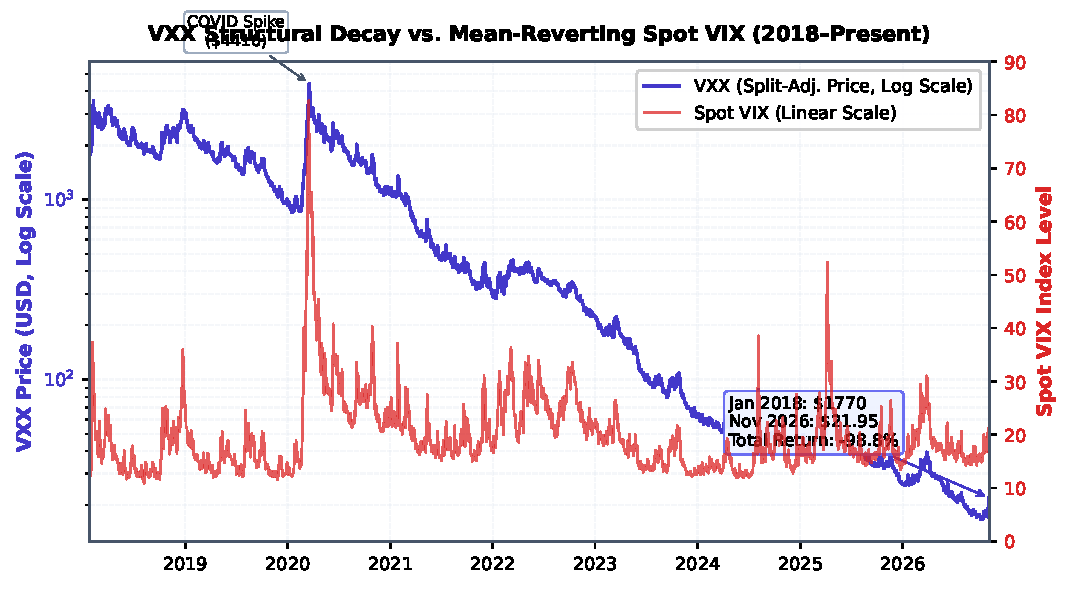
\includegraphics[width=0.9\linewidth]{figures/vxx_vs_vix.pdf}
  \caption{VXX decays over time despite a mean-reverting VIX. This persistent loss reflects negative roll yield caused by contango in the futures curve (split-adjusted price, log scale). Data: Yahoo Finance.}
  \label{fig:vxx}
\end{figure}

\subsubsection{Inverse and leveraged products}

Inverse products such as XIV and SVXY take the opposite side: they earn the roll yield in contango but lose when volatility spikes. Because leveraged and inverse products reset their exposure \emph{daily}, their return over several days is path-dependent. If the underlying futures return is $r$ over one day, a $-1\times$ inverse product's net asset value is multiplied by
\begin{equation}
  1 - r .
  \label{eq:inverse}
\end{equation}
A one-day futures rise of $r\geq 100\%$ would therefore wipe the product out entirely, and a rise of $r=90\%$ would leave only $10\%$ of its value.

There is also a mechanical feedback effect. To restore $-1\times$ exposure at the close after a spike, an inverse product must \emph{buy} VIX futures, which adds to the very rally that caused the losses \cite{augustin}.

\subsection{Volmageddon (February 2018)}
\subsubsection{Background}

After a long period of low volatility, with the VIX near 9--12 in late 2017, short-volatility strategies had been extremely profitable and inverse VIX ETPs such as XIV and SVXY had grown large, holding about \$3.6~billion between them on 5 February 2018 \cite{bbgvol}. This set the stage for a violent reversal.

\subsubsection{Timeline}

\begin{table}[H]
\centering
\small
\begin{tabular}{@{}p{3.6cm}p{11cm}@{}}
\toprule
\textbf{Date} & \textbf{Event}\\
\midrule
Late Jan.--2 Feb.\ 2018 & Equity sell-off begins after a strong January rally\\
5 Feb.\ 2018 & S\&P~500 falls about 4\%; VIX roughly doubles in a day (+115.6\%), its largest one-day percentage rise on record\\
5 Feb.\ 2018, after close & XIV's indicative value falls by 96\% (from \$108.37 to \$4.22)\\
6--21 Feb.\ 2018 & Issuer (Credit Suisse) accelerates (6 Feb.) and terminates XIV (final cash settlement on 21 Feb.) \cite{csxiv}\\
\bottomrule
\end{tabular}
\caption{Key events of the Volmageddon episode.}
\label{tab:timeline}
\end{table}

\subsubsection{Why the products broke}

Three mechanisms combined:
\begin{enumerate}
  \item \textbf{Short exposure to a bounded-below, unbounded-above variable.} By~\eqref{eq:inverse}, a large rise in VIX futures implies a loss approaching 100\% for an inverse product in a single day.
  \item \textbf{Daily rebalancing feedback.} Buying futures near the close to restore exposure amplified the spike in futures prices \cite{augustin}.
  \item \textbf{Termination provisions.} The XIV notes allowed the issuer to accelerate the product if the indicative value fell by 80\% or more in one day (specifically, if intraday indicative value was $\le 20\%$ of the previous day's close) \cite{csxiv}.
\end{enumerate}

\begin{figure}[H]
  \centering
  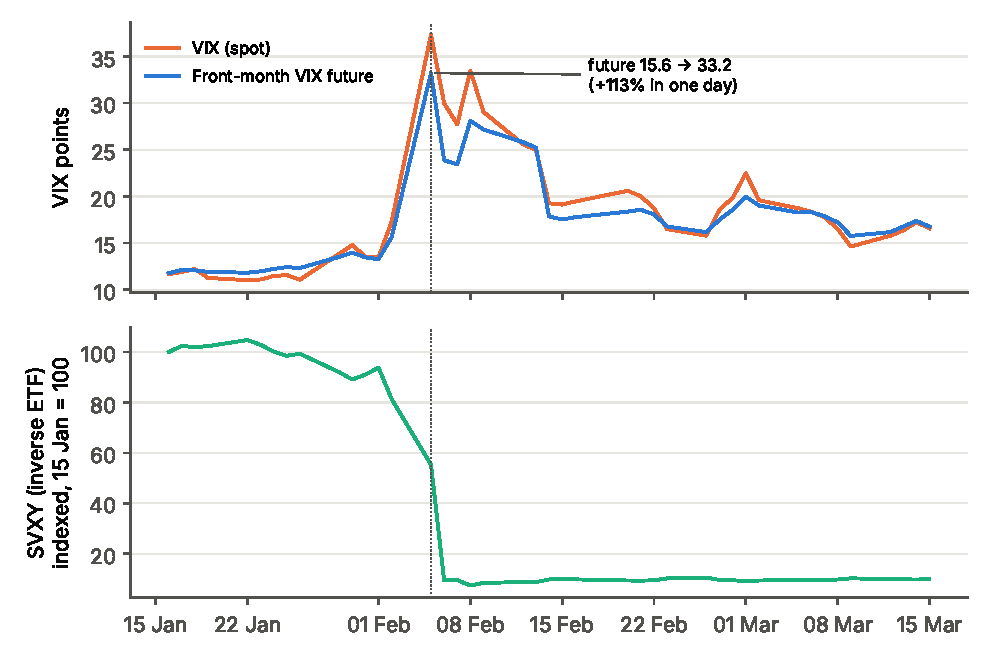
\includegraphics[width=0.9\linewidth]{figures/volmageddon.pdf}
  \caption{Top: VIX and the front-month VIX future, 15 January -- 15 March 2018; on 5 February the front-month future rose from 15.6 to 33.2. Bottom: the inverse VIX ETF SVXY, indexed to 100 on 15 January. Data: Yahoo Finance, Cboe Futures Exchange settlement prices.}
  \label{fig:volmageddon}
\end{figure}

\subsubsection{Aftermath and lessons}

After the event, regulators and exchanges paid closer attention to leveraged and inverse ETPs, and surviving products were redesigned (for example, SVXY reduced its target exposure from $-1.0\times$ to $-0.5\times$) \cite{proshares}. The main lessons are: (i) selling volatility earns a premium but carries severe crash risk; (ii) daily-reset products are path-dependent and unsuitable for buy-and-hold; and (iii) the structure of a product, including issuer risk and termination clauses, matters as much as its underlying exposure.

\subsection{Link to the Rest of the Report}
The next sections specify the VIX methodology and futures contract in detail, including the term structure (contango versus backwardation); derive $\VIX^2$ as the fair strike of a 30-day variance swap and quantify the convexity adjustment; and implement the Cboe formula, a Heston simulation and a backtest of a VIX-futures hedge including roll yield.
